\documentclass[18pt]{ctexart}
% ctexart 自带的边距太大了费纸
% 格式要求里写最好不超过 20 页
\newcommand{\prb}{\times 10^5~\mathrm{kPa}}
\newcommand{\pre}{~\mathrm{kPa}}
\newcommand{\vol}{~\mathrm{mm^3}}
\newcommand{\are}{~\mathrm{mm^2}}
\newcommand{\len}{~\mathrm{mm}}
\newcommand{\tim}{~\mathrm{ms}}
\newcommand{\vel}{~\mathrm{ms^{-1}}}
\newcommand{\mas}{~\mathrm{mg}}
\newcommand{\den}{~\mathrm{mg~mm^{-3}}}
\usepackage[hmargin=3cm,vmargin=4cm]{geometry}
\usepackage{xcolor}
\usepackage{booktabs}
\usepackage{tikz}
\usetikzlibrary{datavisualization}
\usetikzlibrary{datavisualization.formats.functions}
\usepackage{amsmath}
\usepackage{lmodern}
\usepackage{graphicx}
\setmainfont{Times New Roman}
% 配置代码高亮
\usepackage{listings}
\lstset{
    basicstyle          =   \sffamily,          % 基本代码风格
    keywordstyle        =   \bfseries,          % 关键字风格
    commentstyle        =   \rmfamily\itshape,  % 注释的风格,斜体
    stringstyle         =   \ttfamily,  % 字符串风格
    flexiblecolumns,                % 别问为什么,加上这个
    numbers             =   left,   % 行号的位置在左边
    showspaces          =   false,  % 是否显示空格,显示了有点乱,所以不现实了
    numberstyle         =   \zihao{-5}\ttfamily,    % 行号的样式,小五号,tt等宽字体
    showstringspaces    =   false,
    captionpos          =   t,      % 这段代码的名字所呈现的位置,t指的是top上面
    frame               =   lrtb,   % 显示边框
}

\lstdefinestyle{Python}{
    language        =   Python, % 语言选Python
    basicstyle      =   \zihao{-5}\ttfamily,
    numberstyle     =   \zihao{-5}\ttfamily,
    keywordstyle    =   \color{blue},
    keywordstyle    =   [2] \color{teal},
    stringstyle     =   \color{magenta},
    commentstyle    =   \color{red}\ttfamily,
    breaklines      =   true,   % 自动换行,建议不要写太长的行
    columns         =   fixed,  % 如果不加这一句,字间距就不固定,很丑,必须加
    basewidth       =   0.5em,
}
\begin{document}
% 取消 ctexart 的页眉标题,并把页码移到页脚
\pagestyle{plain}
\title{标题}
% 不能添加作者,最后输出文档时应该把下一行注释掉,写在这里是防 warning
\author{}
% 不需要日期,不过如果不这么设置 ctexart 会自动加上 today
\date{}
\maketitle
\section*{摘要}

本文不包含前两页(承诺书 + 评审表格),这是因为每年前两页的内容都可能有变化;而且在所提供的 Word 上填写比设计 \LaTeX 样式容易得多\cite{someitem}。为此也将本文中的字体从 \verb|ctexart| 默认的 Computer Modern Roman 改成了 Times New Roman。

摘要第二段。

\paragraph*{关键词} 关键词一\quad 关键词二
\newpage
\section{问题的重述}
\subsection{引言}
燃油进入和喷出高压油管是许多燃油发动机工作的基础,图 1 给出了某高压 燃油系统的工作原理,燃油经过高压油泵从 A 处进入高压油管,再由喷口 B 喷 出。燃油进入和喷出的间歇性工作过程会导致高压油管内压力的变化,使得所喷 出的燃油量出现偏差,从而影响发动机的工作效率。

\begin{figure}[h]
    \centering
    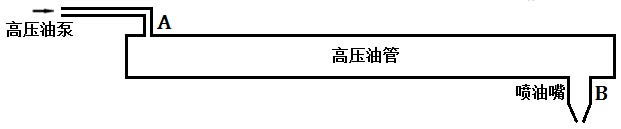
\includegraphics[scale = 1.2]{sketch.jpg}
    \caption{高压油管示意图}
\end{figure}

\subsection{问题的提出}
\subsubsection{问题一}
某型号高压油管的内腔长度为 500mm,内直径为 10mm,供油入口
A 处小孔的直径为 1.4mm,通过单向阀开关控制供油时间的长短,单向阀每打开 一次后就要关闭 10ms。喷油器每秒工作 10 次,每次工作时喷油时间为 2.4ms, 喷油器工作时从喷油嘴 B 处向外喷油的速率如图 2 所示。高压油泵在入口 A 处 提供的压力恒为 160 MPa,高压油管内的初始压力为 100 MPa。如果要将高压油 管内的压力尽可能稳定在 100 MPa 左右,如何设置单向阀每次开启的时长?如 果要将高压油管内的压力从 100 MPa 增加到 150 MPa,且分别经过约 2 s、5 s 和 10 s 的调整过程后稳定在 150 MPa,单向阀开启的时长应如何调整?

用自己的话将问题重述一遍,描述清楚问题涉及的范围,输入信息和输出信息。
\newpage
\section{问题的分析}
\subsection{问题一的分析}
\subsubsection{第一问}
问题一的第一问要求我们通过设置单向阀每次开启的时长,来使得高压油管内的压力稳定在 $1\prb$。由题目所给信息,在喷油器的一个工作周期($100\tim$)内,喷油器喷出的油量为 $44\vol$,而油管的容积为 $3.93\times 10^4\vol$,可见油管中的油量变化在 $0.1\%$ 上下,可以近似认为压强不变。

在一个工作周期内,喷油器喷出的流量已知;且在压强不变的近似下,单向阀流入的流速也已知,因而我们可以根据质量守恒定律列出一个工作周期内单向阀应当开启的时间,进行等比例转换后即能得到单向阀每次开启的时间。

在上述讨论过程中,忽略了高压油管内的压强变化,并且忽略了同一时间段内单向阀和喷油器的相互影响,这一影响的大小可以通过对体系进行精确的数值模拟来考察。在数值模拟中,我们采取较小的时间步长(如 $0.01\tim$),在每一步完成以下计算:

\begin{enumerate}
    \item 检查该时刻单向阀是否处于开启状态;
    \item 如果开启,根据两边压强计算单向阀流入的流量;
    \item 检查该时刻喷油嘴是否处于开启状态;
    \item 如果开启,根据题目所给的流速随时间变化关系计算喷油嘴流出的流量;
    \item 将出入流量乘以相应密度换算为高压油管内燃油的质量变化,进而计算得到更新后的油管内燃油密度;
    \item 将油管内燃油密度的变化通过弹性模量转化为油管内压强的变化;
    \item 将上一步得到的压强继续用于下一步的计算。
\end{enumerate}

通过数值模拟方法,我们可以得到任意时刻油管内的压强,进而计算压强相对于 $1\prb$ 的偏离幅度大小,进而验证我们通过质量守恒定律选取的开启时间是否是使得系统偏离幅度大小最小的开启时间。
\subsection{问题二的分析}
\subsection{问题三的分析}
\newpage
\section{模型的建立与求解}
\subsection{符号说明}


\begin{table}[!ht]
    \begin{minipage}{\textwidth}
        \begin{minipage}[t]{0.5\textwidth}
        \centering
        \caption{符号说明}
        \begin{tabular}{cc}
        \toprule
        符号             & 物理量           \\
        \midrule
        $P_1$          & 油泵压力          \\
        $V_1$          & 油泵体积          \\
        $\rho_1$       & 油泵中燃油密度       \\
        $P_2$          & 油管压力          \\
        $P_2^*$        & 目标油管压力        \\
        $d_2$          & 油管直径          \\
        $l_2$          & 油管长度          \\
        $V_2$          & 油管体积          \\
        $\rho_2$       & 油管中燃油密度       \\
        $d_A$          & A 处小孔直径       \\
        $S_A$          & A 处小孔面积       \\
        $Q_A$          & A 处小孔流量       \\
        $d_B$          & B 处喷孔直径       \\
        $S_B$          & B 处喷孔直径       \\
        $Q_B$          & B 处喷油嘴流量      \\
        $\tau_0$       & 油管的喷油周期       \\
        $\tau_A$       & 喷油周期内 A 的开启时间 \\
        $\tau_A^+$     & A 每次的开启时间     \\
        $\tau_A^-$     & A 每次的关闭时间     \\
        $\tau_A^{\pm}$ & A 一次开启/关闭的总时间 \\
        $\theta$       & 凸轮各点极角        \\
        $\alpha$       & 凸轮极轴方位角       \\
        $h$            & 凸轮最高点高度       \\
        $\omega$       & 凸轮角速度         \\
        $\gamma$       & 圆锥半角          \\
        $z$            & 针阀高度          \\ \bottomrule
        \end{tabular}
        \end{minipage}
        \begin{minipage}[t]{0.5\textwidth}
        \centering
        \caption{符号说明}
        \begin{tabular}{cc}
        \toprule
        符号             & 物理量           \\
        \midrule
        $P_1$          & 油泵压力          \\
        $V_1$          & 油泵体积          \\
        $\rho_1$       & 油泵中燃油密度       \\
        $P_2$          & 油管压力          \\
        $P_2^*$        & 目标油管压力        \\
        $d_2$          & 油管直径          \\
        $l_2$          & 油管长度          \\
        $V_2$          & 油管体积          \\
        $\rho_2$       & 油管中燃油密度       \\
        $d_A$          & A 处小孔直径       \\
        $S_A$          & A 处小孔面积       \\
        $Q_A$          & A 处小孔流量       \\
        $d_B$          & B 处喷孔直径       \\
        $S_B$          & B 处喷孔直径       \\
        $Q_B$          & B 处喷油嘴流量      \\
        $\tau_0$       & 油管的喷油周期       \\
        $\tau_A$       & 喷油周期内 A 的开启时间 \\
        $\tau_A^+$     & A 每次的开启时间     \\
        $\tau_A^-$     & A 每次的关闭时间     \\
        $\tau_A^{\pm}$ & A 一次开启/关闭的总时间 \\
        $\theta$       & 凸轮各点极角        \\
        $\alpha$       & 凸轮极轴方位角       \\
        $h$            & 凸轮最高点高度       \\
        $\omega$       & 凸轮角速度         \\
        $\gamma$       & 圆锥半角          \\
        $z$            & 针阀高度          \\ \bottomrule
        \end{tabular}
        \end{minipage}
    \end{minipage}
\end{table}

本文中,所有长度均以 $\mathrm{mm}$ 为单位,所有质量均以 $\mathrm{mg}$ 为单位,所有时间均以 $\mathrm{ms}$ 为单位。由于压强的量纲为 $\mathrm{ML^{-1}T^{-2}}$,当使用上述三个基本力学量的单位时,压强的自然单位是 $\mathrm{kPa}$,因此本文中所有压强均以 $\mathrm{kPa}$ 为单位。

\subsection{问题一的求解}

\subsubsection{数据预处理}

为考察系统在不同压力下的行为,首先要建立压力和燃油密度的函数关系。但题目中只给出了压力与弹性模量的关系,因此我们通过数据预处理的步骤将它转化为所需要的数据形式。

由题意,燃油的压力变化量与密度变化量成正比,比例系数为 $E/\rho$,且已知 $P^*=1\prb$ 对应着,$\rho^* = 0.850\den$。据此我们可以列出如下的微分方程:

$$
\frac{\mathrm dP}{\mathrm d\rho}=\frac{E}{\rho}
$$

由于题目中将 $E$ 表示为 $P$ 的函数,我们进行移项并积分,得到:

$$
\int_{P^*}^{P'}\frac{\mathrm dP}{E(P)}=\int_{\rho^*}^{\rho'}\frac{\mathrm d\rho}{\rho}=\ln\rho'-\ln\rho^*
$$

但对于函数 $E(P)$ 我们只知道有限个点的函数值,因此左方的积分必须通过数值积分的方法计算,为此我们首先选取上限 $P' = 1.005\prb$,将左方的积分近似表示为 $(E(P^*)^{-1}+E(P')^{-1})/2$,而这两点处的函数值均已知,进而右方的 $\rho'$ 可以从上式中解出。依此类推,每次积分 $500\pre$ 的区间,逐次迭代得到若干个 $\rho'$ 的函数值直至 $2\prb$,再向反方向逐次迭代直至 $0$,即得到所需的函数关系。

\subsubsection{第一小问}
\paragraph{理论计算}
首先假设油管的压力近似保持在 $P_2=P_2^*=1.00\prb$,因而油管内燃油 密度 $\rho_2$ 为常数。在喷油器的一个工作周期内,从喷油嘴流出的燃油质量,由流速对时间的积分与密度的乘积给出:

$$
\Delta m=\int_0^{\tau_0}Q_B\rho_2\mathrm dt=37.4\mas
$$

这些质量应当由从单向阀进入的燃油补充,因此在喷油器一个工作周期内,单向阀平均应该开启的时间应当由损失的质量和补充燃油质量的速度决定:

$$
\begin{aligned}
\tau_A&=\frac{\Delta m}{Q_A\rho_1}\\
&=\frac{\Delta m}{\rho_1CA\sqrt{2(P_1-P_2)/\rho_1}}\\
&=2.76\tim
\end{aligned}
$$

若我们考虑系统进行较长时间的演化,则在一个周期内单向阀平均开启的时间应该与相同。因此,单向阀开启的时长 $\tau_A^+$ 与它关闭的时长 $\tau_A^-$ 应该满足如下比例式:

$$
\frac{\tau_A^+}{\tau_A^-}=\frac{\tau_A}{\tau_0-\tau_A}
$$

代入已知数据,可以求出 $\tau_A=0.284\tim$。

\paragraph{数值模拟}

在数值模拟中,我们设定初始条件为 $P_2=1.00\prb$,且时间零点恰好位于喷油器一个工作周期的开始,但可以位于单向阀一个工作周期中的任意一点,该点处相位为 $t_0$。

系统的演化可以用如下关系表示,其中左箭头「$\leftarrow$」是程序设计中的赋值等号:

$$
\begin{aligned}
    Q_A &\leftarrow Q_A(t)\\
    m_2 &\leftarrow m_2 + Q_A \times \rho_1 \times dt\\
    Q_B &\leftarrow Q_B(t)\\
    m_2 &\leftarrow m_2 - Q_B \times \rho_2 \times dt\\
    \rho_2 &\leftarrow m_2 / V_2\\
    P_2 &\leftarrow P(\rho_2)\\
\end{aligned}
$$

将系统进行 $N$ 个周期的演化,获得各个时刻油管的压强后,我们可以定义系统关于目标压力的均方根偏差 $D$ 作为压强-时间函数的泛函:

$$
D[P_2(t)]=\sqrt{\frac1{N\tau_0}\int_0^{N\tau_0}
\left[P_2(t)-P_2^*\right]^2\mathrm dt}
$$

给定一系列开启时间 $\tau_A^+$,计算它们的均方根偏差,就可以从中找出使得均方根偏差最小的开启时间。
\subsection{第二小问}
我们可以通过与第一小问中相同的方法,来近似计算令油管压力稳定在 $1.5\prb$ 所需要的开启时间,结果为 $\tau_A^+ = 0.759\tim$。根据第一小问中的结论,这一时间就是在当模拟时间趋于 $+\infty$ 时,使油管压力关于目标压力的均方根偏差最小的开启时间。

因此,我们可以只考虑分别在 $2000, 5000, 10000\tim$ 的调整过程中应该令 $\tau_A^+$ 为多大。由于这一过程中油管压力发生了显著的变化,不能近似认为压力不变,因此难于解析求解。我们仍采用数值模拟的方法,通过扫描一个大致含有最佳 $\tau_A^+$ 的时间范围来确定最佳的 $\tau_A^+$。计算结果如图所示:

(插入图片)

由此可见,调整过程分别为 $2000, 5000, 10000\tim$ 时,最佳的 $\tau_A$ 分别为 XXX、XXX 和 XXX。
\subsection{问题二}
\subsubsection{数据预处理}
由题意,高压油泵通过柱塞实现向外压油,柱塞由凸轮驱动上下运动,且已知凸轮边缘曲线与角度的关系,因此首先要将凸轮边缘曲线转化为柱塞的高度。

当凸轮极轴的方位角为 $\alpha$ 时,凸轮上极角 $\theta$ 的方向对应的方位角为 $\alpha + \theta$。因此,我们可以选取一系列 $\alpha$ 的数据点 $\alpha_i$,在每个数据点处遍历所有的极角 $\theta_j$,计算对应极径的实际高度并取最大值,作为柱塞的高度:

$$
h(\alpha_i)=\max_j(r_j\times \sin(\alpha_i+\theta_j))
$$

再对上述数据点处的高度 $h$ 进行线性内插即得到函数 $h(\alpha)$。
\subsubsection{锥形喷油器流速的求解}

题目中未给出喷油器的流速,因此需要利用密封座的几何参数进行求解。根据已知信息可以定量画出喷油器:

由此看出,在喷油的过程中,针阀以下的部分形成了一个较大的空间,其体积至少为

$$
\frac{\pi}{24}\cot\gamma\times\left(d_I^3-d_B^3\right)\approx 10\vol
$$

而该部分体积与上下均有隔离,因此喷油过程可以用两次扩散过程进行近似。到达稳态时,两次扩散的流速相同,由此对喷嘴可以列出以下方程:

$$
\begin{aligned}
Q=S_B'\sqrt{\frac{2(P_2-P_3)}{\rho_2}}=S_B\sqrt{\frac{2(P_3-P_0)}{\rho_3}}
\end{aligned}
$$

其中等效面积 $S_B'$ 的物理意义是从油管扩散到缓冲区时,计算公式为:

$$
\frac{1}{2}\pi{}(d+2l\cos{\gamma})(l+r)-\frac{1}{2}\pi{}dr = \pi^2(h^2\sin{\gamma}^2\cos{\gamma}+dz\sin{\gamma})
$$

通过该方程可以求出给定压强 $P_2$ 和给定针阀升程 $z$ 下的流量 $Q_B$。

\subsubsection{数值模拟}

我们仍以均方误差为判据,考察不同角速度下关于目标压力的均方根偏离 $D$:

(图片 ../2/D-omega.dat)

由此可见 $\omega=0.0256\vel$ 为最优的角速度。在该角速度下,系统

% \begin{figure}
%     \begin{minipage}[t]{\textwidth}
%         \begin{minipage}[t]{0.33\textwidth}
%         \end{minipage}
%         \begin{minipage}[t]{0.33\textwidth}
%         \end{minipage}
%         \begin{minipage}[t]{0.33\textwidth}
%         \end{minipage}
%     \end{minipage}
% \end{figure}
\newpage
\section{模型的评价}
优点、缺点、潜在改进空间和应用范围。
\newpage
\begin{thebibliography}{100}
\bibitem{someitem} 作者.题目[J].期刊,年份,卷(期):起始页-终止页.
\end{thebibliography}
\newpage
\appendix
\section{源代码}
\subsection{说明}
\begin{enumerate}
    \item 本文中全部代码使用 Python 3 编写,并使用 3.7.1 版本的解释器解释运行;
    \item 输入数据以文本文件 \verb|.raw| 
    \item 第一题至第三题每题在设有一个文件夹(如 \verb|1/|);
    \item 第一题有一个模块文件 \verb|EigenProblem.f90| 和三个源代码文件 \verb|1_2.f90|, \verb|1_3.f90| 和 \verb|1_4.f90|;第二题有一个模块文件 \verb|Functions.f90| 和三个源代码文件 \verb|2_1.f90|, \verb|2_2.f90| 和 \verb|2_3.f90|;第三题有两个代码文件 \verb|3_2.f90| 和 \verb|3_3.f90|;每个代码文件对应一个无后缀的可执行文件。
    \item 所有代码文件均无输入文件,也不需要在执行过程中输入;
    \item 所有代码文件均对应输出文件 \verb|<可执行文件名>_output.txt|,提交时已经运行过并生成了相应的输出文件;
    \item XXX 程序运行时间较长
\end{enumerate}
\subsection{模块源代码}
\subsection{第一题源代码}
\subsection{第二题源代码}
\subsection{第三题源代码}
\newpage
\section{其他数据资料}
\end{document}